\iffalse
\documentclass[journal,11pt,twocolumn]{IEEEtran}
\usepackage{setspace}
\usepackage{gensymb}
\singlespacing
\usepackage[cmex10]{amsmath}
\usepackage{amsthm}
\usepackage{mathrsfs}
\usepackage{txfonts}
\usepackage{stfloats}
\usepackage{bm}
\usepackage{cite}
\usepackage{cases}
\usepackage{subfig}
\usepackage{longtable}
\usepackage{multirow}
\usepackage{enumitem}
\usepackage{mathtools}
\usepackage{tikz}
\usepackage{circuitikz}
\usepackage{verbatim}
\usepackage[breaklinks=true]{hyperref}
\usepackage{tkz-euclide} % loads  TikZ and tkz-base
\usepackage{listings}
\usepackage{color}    
\usepackage{array}    
\usepackage{longtable}
\usepackage{calc}     
\usepackage{multirow} 
\usepackage{hhline}   
\usepackage{ifthen}   
\usepackage{lscape}     
\usepackage{chngcntr}
\usepackage{float}
\DeclareMathOperator*{\Res}{Res}
\renewcommand\thesection{\arabic{section}}
\renewcommand\thesubsection{\thesection.\arabic{subsection}}
\renewcommand\thesubsubsection{\thesubsection.\arabic{subsubsection}}

\renewcommand\thesectiondis{\arabic{section}}
\renewcommand\thesubsectiondis{\thesectiondis.\arabic{subsection}}
\renewcommand\thesubsubsectiondis{\thesubsectiondis.\arabic{subsubsection}}
\renewcommand\thetable{\arabic{table}}
% correct bad hyphenation here
\hyphenation{op-tical net-works semi-conduc-tor}
\def\inputGnumericTable{}                                 %%

\lstset{
%language=C,
frame=single, 
breaklines=true,
columns=fullflexible
}
%\lstset{
%language=tex,
%frame=single, 
%breaklines=true
%}
\providecommand{\pr}[1]{\ensuremath{\Pr\left(#1\right)}}
\providecommand{\prt}[2]{\ensuremath{p_{#1}^{\left(#2\right)} }}        % own macro for this question
\providecommand{\qfunc}[1]{\ensuremath{Q\left(#1\right)}}
\providecommand{\sbrak}[1]{\ensuremath{{}\left[#1\right]}}
\providecommand{\lsbrak}[1]{\ensuremath{{}\left[#1\right.}}
\providecommand{\rsbrak}[1]{\ensuremath{{}\left.#1\right]}}
\providecommand{\brak}[1]{\ensuremath{\left(#1\right)}}
\providecommand{\lbrak}[1]{\ensuremath{\left(#1\right.}}
\providecommand{\rbrak}[1]{\ensuremath{\left.#1\right)}}
\providecommand{\cbrak}[1]{\ensuremath{\left\{#1\right\}}}
\providecommand{\lcbrak}[1]{\ensuremath{\left\{#1\right.}}
\providecommand{\rcbrak}[1]{\ensuremath{\left.#1\right\}}}
\newcommand{\sgn}{\mathop{\mathrm{sgn}}}
\providecommand{\abs}[1]{\left\vert#1\right\vert}
\providecommand{\res}[1]{\Res\displaylimits_{#1}} 
\providecommand{\norm}[1]{\left\lVert#1\right\rVert}
%\providecommand{\norm}[1]{\lVert#1\rVert}
\providecommand{\mtx}[1]{\mathbf{#1}}
\providecommand{\mean}[1]{E\left[ #1 \right]}
\providecommand{\cond}[2]{#1\middle|#2}
\providecommand{\fourier}{\overset{\mathcal{F}}{ \rightleftharpoons}}
%\providecommand{\hilbert}{\overset{\mathcal{H}}{ \rightleftharpoons}}
%\providecommand{\system}{\overset{\mathcal{H}}{ \longleftrightarrow}}
	%\newcommand{\solution}[2]{\textbf{Solution:}{#1}}
\newcommand{\solution}{\noindent \textbf{Solution: }}
\newcommand{\cosec}{\,\text{cosec}\,}
\providecommand{\dec}[2]{\ensuremath{\overset{#1}{\underset{#2}{\gtrless}}}}
\newcommand{\myvec}[1]{\ensuremath{\begin{pmatrix}#1\end{pmatrix}}}
\newcommand{\mydet}[1]{\ensuremath{\begin{vmatrix}#1\end{vmatrix}}}
\providecommand{\rank}{\text{rank}}
\providecommand{\pr}[1]{\ensuremath{\Pr\left(#1\right)}}
\providecommand{\qfunc}[1]{\ensuremath{Q\left(#1\right)}}
	\newcommand*{\permcomb}[4][0mu]{{{}^{#3}\mkern#1#2_{#4}}}
\newcommand*{\perm}[1][-3mu]{\permcomb[#1]{P}}
\newcommand*{\comb}[1][-1mu]{\permcomb[#1]{C}}
\providecommand{\qfunc}[1]{\ensuremath{Q\left(#1\right)}}
\providecommand{\gauss}[2]{\mathcal{N}\ensuremath{\left(#1,#2\right)}}
\providecommand{\diff}[2]{\ensuremath{\frac{d{#1}}{d{#2}}}}
\providecommand{\myceil}[1]{\left \lceil #1 \right \rceil }
\newcommand\figref{Fig.~\ref}
\newcommand\tabref{Table~\ref}
\newcommand{\sinc}{\,\text{sinc}\,}
\newcommand{\rect}{\,\text{rect}\,}
\title{Assignment}
\author{Barath surya M | EE22BTECH11014}
\begin{document}
\newtheorem{theorem}{Theorem}[section]
\newtheorem{problem}{Problem}
\newtheorem{proposition}{Proposition}[section]
\newtheorem{lemma}{Lemma}[section]
\newtheorem{corollary}[theorem]{Corollary}
\newtheorem{example}{Example}[section]
\newtheorem{definition}[problem]{Definition}
\newcommand{\BEQA}{\begin{eqnarray}}
\newcommand{\EEQA}{\end{eqnarray}}
\newcommand{\define}{\stackrel{\triangle}{=}}
\bibliographystyle{IEEEtran}
\providecommand{\mbf}{\mathbf}
\providecommand{\pr}[1]{\ensuremath{\Pr\left(#1\right)}}
\providecommand{\qfunc}[1]{\ensuremath{Q\left(#1\right)}}
\providecommand{\sbrak}[1]{\ensuremath{{}\left[#1\right]}}
\providecommand{\lsbrak}[1]{\ensuremath{{}\left[#1\right.}}
\providecommand{\rsbrak}[1]{\ensuremath{{}\left.#1\right]}}
\providecommand{\brak}[1]{\ensuremath{\left(#1\right)}}
\providecommand{\lbrak}[1]{\ensuremath{\left(#1\right.}}
\providecommand{\rbrak}[1]{\ensuremath{\left.#1\right)}}
\providecommand{\cbrak}[1]{\ensuremath{\left\{#1\right\}}}
\providecommand{\lcbrak}[1]{\ensuremath{\left\{#1\right.}}
\providecommand{\rcbrak}[1]{\ensuremath{\left.#1\right\}}}
\theoremstyle{remark}
\newtheorem{rem}{Remark}
\providecommand{\abs}[1]{\left\vert#1\right\vert}
\providecommand{\res}[1]{\Res\displaylimits_{#1}} 
\providecommand{\norm}[1]{\left\lVert#1\right\rVert}
\providecommand{\mtx}[1]{\mathbf{#1}}
\providecommand{\mean}[1]{E\left[ #1 \right]}
\providecommand{\fourier}{\overset{\mathcal{F}}{ \rightleftharpoons}}
\providecommand{\system}[1]{\overset{\mathcal{#1}}{ \longleftrightarrow}}
\providecommand{\dec}[2]{\ensuremath{\overset{#1}{\underset{#2}{\gtrless}}}}
\let\vec\mathbf
\def\putbox#1#2#3{\makebox[0in][l]{\makebox[#1][l]{}\raisebox{\baselineskip}[0in][0in]{\raisebox{#2}[0in][0in]{#3}}}}
     \def\rightbox#1{\makebox[0in][r]{#1}}
     \def\centbox#1{\makebox[0in]{#1}}
     \def\topbox#1{\raisebox{-\baselineskip}[0in][0in]{#1}}
     \def\midbox#1{\raisebox{-0.5\baselineskip}[0in][0in]{#1}}
\maketitle
Question Let $X$ be a random variable having poisson distribution with mean $\lambda>0$. Then E\brak{\cond{\frac{1}{1+X}}{X>0}} equals
\begin{enumerate}
	\item $\frac{1-e^{-\lambda}-\lambda e^{-\lambda}}{\lambda\brak{1-e^{-\lambda}}}$
	\item $\frac{1-e^{-\lambda}}{\lambda}$
	\item $\frac{1-e^{-\lambda}-\lambda e^{-\lambda}}{\lambda}$
	\item $\frac{1-e^{-\lambda}}{\lambda +1}$
\end{enumerate}

\solution
\\
\fi
\begin{enumerate}[label=(\Alph*)]
	\item Theory
\begin{align}
	X&\sim Pois\brak{\lambda}\\
	\pr{X=k}&=e^{-\lambda} \frac{\lambda^k}{k!}; k \geq 0 \label{eq:poissondistributionpmf}
\end{align}
we know that 
\begin{align}
	E\brak{A|B}&=\frac{E\brak{A,B}}{\pr{B}}\\
	\implies E\brak{\cond{\frac{1}{1+X}}{X>0}} &=\frac{\sum_{k=1}^{\infty}\frac{1}{k+1}\pr{X=k}}{\pr{X>0}}\\
	&=\frac{\sum_{k=1}^{\infty}\frac{1}{k+1} e^{-\lambda}\frac{\lambda^k}{k!}}{1-\pr{X\leq 0}}\\
	&=\frac{e^{-\lambda}\sum_{k=1}^{\infty}\frac{\lambda^k}{\brak{k+1}!}}{1-\pr{X=0}}
\end{align}
from equation \eqref{eq:poissondistributionpmf}
\begin{align}
	&=\frac{e^{-\lambda}\sum_{k=1}^{\infty}\frac{\lambda^k}{\brak{k+1}!}}{1-e^{\lambda}}
\end{align}
Now simplifying Just the Summation
\begin{align}
	\implies & \sum_{k=1}^{\infty} \frac{\lambda^k}{\brak{k+1}!}\\
	&=\frac{1}{\lambda} \sum_{k=1}^{\infty} \frac{\lambda^{k+1}}{k+1}
\end{align}
Letting $k+1 =m $,
\begin{align}
	\implies & \frac{1}{\lambda} \sum_{m=2}^{\infty} \frac{\lambda^m}{m!}
\end{align}
We Know from Taylor series
\begin{align}
	e^x&=\sum_{k=0}^{\infty} \frac{x^k}{k!}\\
	\implies \frac{1}{\lambda} \sum_{m=2}^{\infty} \frac{\lambda^m}{m!}&= \frac{1}{\lambda}\brak{e^{\lambda}-1-\lambda}
\end{align}
Substituting back we get,
\begin{align}
	&=\frac{e^{-\lambda}}{ \brak{1-e^{\lambda}}}\brak{\frac{1}{\lambda} \brak{e^{\lambda}-1-\lambda}}\\
	&=\frac{e^{-\lambda}}{\lambda \brak{1-e^{\lambda}}}\brak{e^{\lambda}-1 -\lambda}\\
	&=\frac{1-e^{-\lambda}-\lambda e^{-\lambda}}{\lambda \brak{1-e^{\lambda}}}
\end{align}
\item Simulation\\
\begin{enumerate}[label=(\roman*)]
	\item In the code, it simulates the generation of RV $X$ using the CDF of Poisson distribution.\\
	\begin{align}
		F\brak{x}&=\sum_{k=0}^{x}e^{-\lambda}\frac{\lambda^k}{k!}
	\end{align}
	\item initialize $X=0$
	\item initialize $F=e^{-\lambda}$ which is $F\brak{0}$ of a poisson distribution
	\item generate a uniform random variable between 0 and 1
	\item enter the loop that continues as long as $u>F$\\
	Inside the loop,
	\item Increment $X$ by 1
	\item Add next term of Poisson pmf $\brak{\pr{X=k+1}}$ to $F\brak{x}$
	\item the loop continues until $u$ is no longer greater than $F$. At this point, X represents the generated value of the poisson random variable that follows the desired poisson distribution with mean parameter $\lambda$.
	\item Save all the values of poisson random variable $X$ in pois.dat so to open it in python an plot the cdf graph 
	\item Then for the second part Check if the generated value of $X$ is greater than 0. If $X$ is greater than 0, calculate the value $Y$ as $\frac{1}{X + 1}$ and add it to the sumY.Increment the validCount to keep track of valid $X$ values.
	\item If validCount is greater than 0, calculate the  estimate of the conditional expectation by dividing sumY by validCount.

\end{enumerate}
\end{enumerate}
\begin{figure}[ht!]
	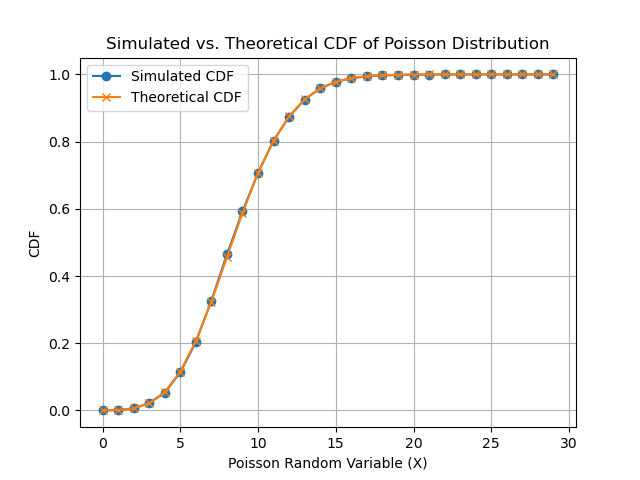
\includegraphics[width=\columnwidth]{2023/ST/17/figs/poisson.png}
	\label{gate17_2023_poissoncdf}
	\caption{Simulation Vs theoretical cdf of poisson distribution with $\lambda=9$}
\end{figure}

